\documentclass{article}
\usepackage{graphicx}
\usepackage{fullpage}
\usepackage{hyperref}

%\usepackage{fontspec}
%\setmainfont{Times New Roman}

\begin{document}

\title{NDN MOG Project Snapshot}
\author{Zening Qu}
\maketitle

\abstract
To be filled.

\tableofcontents
\listoffigures
\listoftables
\newpage

%-------------------------------------------------------------------------------------------------------------------------------------%
% Introduction
%-------------------------------------------------------------------------------------------------------------------------------------%
\section{Introduction: Objective, Potential Findings}
\label{itro}
%Massively Multiplayer Online Games (MMOGs) are gaining research attention these years. The LPP project is an exploration of the design and creation of such games on Named Data Network (NDN). The {consistency}, scalability, availability and security issues of MMOG design are of special interest. As of genre and gameplay, we are interested in creating an Role Playing Game (RPG) inspired by \emph{Le Petit Prince}, which is how this project got its name.

%This document is a snapshot of the current progress of the LPP project. It is aimed for the research group to reflect on the finished work and plan the next steps. It contains an in-progress survey of MMOG design issues in the IP world (section \ref{bg}), a brief description of our previous NDN car racing game (section \ref{prew}) and designs of LPP which is our logical next step (section \ref{nstp}). 

% Define the document, Intended readers
This document is aimed for the Named Data Networking Multiplayer Online Game (NDN MOG) research group. It is written at a time when a small scale car racing game was implemented and synchronized on the NDN testbed \cite{egalcar}. The author tries to provide a rich background of Peer-to-Peer MOG design, in the hope of fostering the design and evaluation of a more extensive Role Playing Game (RPG) game over NDN. On the other hand, the author does not attempt to bring up too much details about NDN. Interested readers should turn to the project website (\href{http://www.named-data.net/}{http://www.named-data.net/}) and its publication list.

%subject to change as we write on
In this section we define the project objective and potential findings. Section \ref{ggd} introduces the general game design of our planned RPG game and compares it with characteristics of World of Warcraft (WoW), the representative MOG. The MOG synchronization problem and related design issues are described in section \ref{dfsync}. Finally, section \ref{dslpp} tries to solve the synchronization problem for our RPG game and evaluate the solution. Note that NDN MOG is an on-going project, hence section \ref{dslpp} is merely a best-effort solution for the time being. The document may raise more questions than it answers. Its content (including background and design) is subject to substantial improvement and change.

\subsection{Project Objectives: Explore The P2P Game Synchronization Problem And The Related Problems}
The primary objective is to explore the Peer-to-Peer (P2P) game synchronization problem on NDN. Closely related problems such as architecture choice, interactivity and scalability are seriously considered. Other related problems like availability and security are taken into account whenever possible. These problems are depicted in section \ref{dfsync}.

\subsection{Project Inspiration: P2P MOGs In The IP World}
In the industry, the Client/Server (C/S) architecture dominant the MOG world. Large MOGs, or Massively Multiplayer Online Games (MMOGs) like World of Warcraft use clusters of servers to handle its thousands of players despite the high cost, service bottleneck and single point-of-failure brought by the centralized servers \cite{Neumann07, Fan10}.

In the academia, there has been debate about P2P architecture's potential for MOGs and MMOGs. Some researchers are very pessimistic: in 2010, Miller et al. predicted that MMOGs with WoW-like scale cannot be deployed using the available P2P scheme \cite{Miller10}. Other researchers find the future of P2P support for MMOGs attractive: in 2004 Knutsson et al. simulated a P2P MOG which scaled up to 4,000 concurrent players \cite{Knutsson04}, and many other P2P schemes were proposed after that \cite{Fan10}. Many researchers agree that the common future of P2P and MMOG remains promising, but for P2P architectures to be a practical alternative of the C/S architecture, many challenges persist: consistency, interactivity, scalability, availability, security etc. \cite{Neumann07, Fan10, Gilmore12}.

P2P game synchronization problem is closely related to these challenges that lay ahead (see section \ref{dfsync}). If the synchronization problem is better solved, P2P MOGs are likely to experience a performance increase. Further, given NDN's many characteristics such as intrinsic multicasting and 

\subsection{Potential Findings: Impact of NDN on P2P MOGs}
% P2P are not favored by the industry, and some researchers are really pessimistic about it
% however, there is hope, Knutsson for example, did a good job in 2004, and NDN has potential to further improve the result. Many researchers are passionate about this topic too.


%-------------------------------------------------------------------------------------------------------------------------------------%
% MMOGs and our Gameplay
%-------------------------------------------------------------------------------------------------------------------------------------%
\section{General Game Design: LPP and WoW}
\label{ggd}
% in this section introduce the gameplay of our prototype game and compare it with WoW.

\subsection{Scale: 1 Million Concurrent Users}

\subsection{Active Entities: Players, NPCs, Mutable Objects}

\subsection{Interactions: Player-Player Interaction, Player-NPC/Object Interaction}

\subsection{Summary: LPP Gameplay}

%-------------------------------------------------------------------------------------------------------------------------------------%
% The Sync Problem
%-------------------------------------------------------------------------------------------------------------------------------------%
\section{The Synchronization Problem and Related Problems}
\label{dfsync}

\subsection{The Consistency Model: Event Based (P2P) and Update Based (C/S)}
% the graph: fully connected P2P model, obviously not scalable (latency is great, but the bandwidth requirement is too high)
% If you want it to scale, you will have to trade great latency for scale
% but you will need a mechanism to limit the latency, like Knutsson did in 2004

\subsubsection{Synchronization Algorithms: Conservative, Optimistic}

\subsection{Related Problems: Architecture, Interactivity, Scalability, Availability, Security}

\subsubsection{Architecture Choice: P2P, C/S, Hybrid}

\subsubsection{Interactivity: MMOGs are Latency-Sensitive}
% the interactivity threshold: 100~150ms
% latency comprises of transmission delay and synchronization delay

\subsubsection{Scalability: P2P Is Scalable, But Not Traditional P2P Consistency Model}
% bandwidth requirement
% I think P2P requires more bandwidth than C/S does, because the central server gathers information effectively
% to reduce bandwidth requirement, we MUST exploit Locality of Interest

\subsubsection{Availability: Robustness of C/S and P2P}
% P2P is better than C/S, but P2P is not perfect 

\subsubsection{Security: P2P Is More Prone To Cheating}
% P2P is more prone to cheating, but C/S is not ideal either

%-------------------------------------------------------------------------------------------------------------------------------------%
% Design of Our Next Planned Game
%-------------------------------------------------------------------------------------------------------------------------------------%
\section{Designing The Next Game: LPP}
\label{dslpp}

\subsection{Namespace}

\begin{figure}[htbp]
\begin{center}
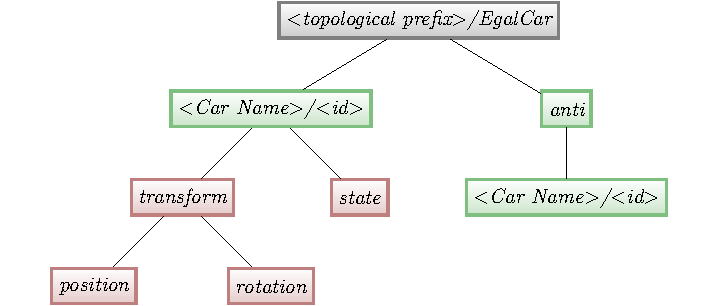
\includegraphics{ObjectTree.pdf}
\caption{Part of LPP's namespace, nodes that contain a ``(sequence number)'' will be explained one by one in this document}
\label{ns}
\end{center}
\end{figure}

\begin{enumerate}
\item \emph{/ndn/ucla.edu/apps/lpp}: the topological prefix of the game
\item \emph{$<$Player ID$>$}: a random number generated in real-time to represent a particular player in the game, this ID is computed in a random manner to (partly) avoid name collisions
\item \emph{$<$Asteroid ID$>$}: a random, real-time number representing a particular asteroid
\item \emph{$<$Seedling ID$>$}: a random, real-time number representing a particular seedling who comes out of a particular asteroid
\item \emph{anti}: this is for asset deletion (publishing an anti-asset corresponds to deleting that particular asset)
\item \emph{.../$<$Player ID$>$/state}: the current state of a particular player; \emph{position} can be used to provide a global view; \emph{experience} can be used to produce a global rank list
\item \emph{.../$<$Asteroid ID$>$/state}: the current state of a particular asteroid, which may contain a name list of all players on that asteroid and things like that
\item \emph{.../$<$Player ID$>$/event}: the action of a particular player
\end{enumerate}

In figure~\ref{ns}, all blue nodes are recognized as \emph{Asset}s, all red nodes \emph{State}s, green ones \emph{Event}s. We will have more documentations about Asset, State, Event in the future. For now it is sufficient to know that these three types of nodes will be synchronized in three different ways.

\subsection{Membership Service and Object Discovery: CCNx Sync}

\subsection{Unreliable, Ordered Delivery of Updates}

\subsection{Reliable, Ordered Delivery of Events}

\subsection{Example of Player-Player Interaction}

\subsection{Example of Player-NPC/Object Interaction}

\subsection{Discussions: Performance}

\bibliographystyle{plain}
\bibliography{MOGRef}
\end{document}